% Write the full path to the location of the graphics relative to book.tex
\graphicspath{{chapters/marcibal/graphics/}}
\title{Implementation of the Lam--Bremhorst \texorpdfstring{$k$-$\varepsilon$}{k-e} Turbulence Model in FEniCS}
\titlerunning{Implementation of the \texorpdfstring{$k$-$\varepsilon$}{k-e} Turbulence Model}
\author{Juraj Marcibál and Hans Joachim Schroll}
\authorrunning{J.~Marcibál, H.~J.~Schroll}
\institute{
J.~Marcibál \email{juraj.marcibal@gmail.com},
H.~J.~Schroll \email{achim@imada.dk}
\at Department of Mathematics and Computer Science, University of Southern Denmark, Odense, Denmark}

\maketitle
% ---- Article starts here ---- 
% Abstract
\abstract{
    In this paper, we give an overview of turbulence modelling and turbulence in general, followed by an implementation of the Lam--Bremhorst $k$-$\varepsilon$ turbulence model in FEniCS.
    We demonstrate how the model can be easily implemented in the latest version of FEniCS, even when working with the simplest methods and schemes.
    We hope this paper serves as a valuable resource for researchers and enthusiasts seeking a straightforward introduction to turbulence modelling and a practical guide for implementing models in FEniCS.
}
    
% Section 1 - Introduction
\section{Introduction and Governing Equations}
Turbulence is an ever-present phenomenon encountered in both natural environments and engineering systems, from airflow over an airplane wing to the movement of water in rivers.
It occurs when fluid moves chaotically, irregularly, and with a high Reynolds number, presenting challenges for study and applications \citep{wilcox_turbulence_2006}.
\subsection{Literature Review}
Turbulence modelling, including the $k$-$\varepsilon$ model and implementation in FEniCS \citep{alnaes2015fenics,baratta2023dolfinx} and other open-source software, has been previously covered in the literature.
The article by \cite{valen_implementing_2013} implements the model by \citep{launder_application_1974}, which is often regarded as the standard $k$-$\varepsilon$ model in FEniCS, providing an accessible introduction to turbulence modelling and FEniCS itself.
However, that code is now over a decade old and covers only a simple channel flow case. On the other hand, \cite{mortensen_fenics-based_2011} present a more comprehensive turbulence modelling framework, implementing multiple models, including the Launder--Sharma $k$-$\varepsilon$ model.
Although it extends beyond the turbulent channel flow example, the code is incompatible with the latest version of legacy FEniCS, and its complexity makes it less approachable for newcomers.
This article aims to address the need for a clear up-to-date turbulence model implementation in legacy FEniCS.
We demonstrate that implementing a turbulence model in the latest version is feasible, and satisfactory results can be obtained even when working with simple numerical schemes and a simpler turbulence model.
Additionally, we provide an introduction to turbulence and turbulence modelling, making this work a valuable starting point for researchers entering the field.

\subsection{Modelling Turbulence}
Consider the incompressible Navier--Stokes (NS) equations
\begin{equation}\label{eq:NS}
    \begin{split}
        \frac{\partial \mathbf{u}}{\partial t} + \mathbf{u} \cdot \nabla{\mathbf{u}}
        =
        - \frac{1}{\rho} \nabla p + \nabla \cdot (\nu \nabla \mathbf{u}) + \mathbf{f},
        \\
        \nabla \cdot \mathbf{u}
        = 0,
    \end{split}
\end{equation}
where $\mathbf{u}$ and $p$ are the instantaneous velocity and pressure, respectively; $\mathbf{f}$ represents external forces; and $\rho$ is the density and $\nu$ is the molecular viscosity of the fluid.
It is well known that solving \cref{eq:NS} numerically becomes difficult with increasing Reynolds numbers.
To accurately predict turbulent flow, we either need to work with a very fine mesh and small step sizes or resort to modelling.
The former is often not feasible without a large amount of computational power.One approach to modelling turbulence is to consider not the instantaneous $\mathbf{u}$ and $p$ but, rather, the mean values $\langle \mathbf{u} \rangle$ and $ \langle p \rangle$.
By decomposing $\mathbf{u}$ and $p$ into their mean and fluctuating parts $\mathbf{u} = \langle \mathbf{u} \rangle + \mathbf{u}'$ and $p = \langle p \rangle + p'$, one can derive governing equations for the mean quantities.
Such equations are called the Reynolds-averaged NS (RANS) equations, and they take the form
\begin{equation}\label{eq:RANS}
    \begin{split}
        \frac{\partial \langle \mathbf{u} \rangle}{\partial t} + \langle \mathbf{u} \rangle \cdot \nabla{\langle \mathbf{u} \rangle}
        = 
        -\frac{1}{\rho} \nabla \langle p \rangle + \nabla \cdot (\nu \nabla \langle \mathbf{u} \rangle ) + \langle \mathbf{f} \rangle - \nabla \cdot \langle \mathbf{u}' \otimes \mathbf{u}' \rangle,
        \\
        \nabla \cdot \langle \mathbf{u} \rangle
        = 0,
    \end{split}
\end{equation}
where $\mathbf{R} := - \langle \mathbf{u}' \otimes \mathbf{u}' \rangle$ is the Reynolds stress tensor, often interpreted as describing the effect of turbulence on the mean flow \citep{wilcox_turbulence_2006}.
It contains $\mathbf{u}'$, which is neither known nor solved for.
The RANS equations are therefore not closed, and $\mathbf{R}$ needs to be modelled, usually using the hypothesis proposed by \cite{boussinesq__essai_1877}:
\begin{equation}\label{eq:Boussinesq_hypothesis}
    \mathbf{R}
    \approx
    - \frac{2}{3}k \mathbf{I}
    + \nu_t \left(\nabla{\mathbf{u}}
    + (\nabla{\mathbf{u}})^T\right)
    \implies
    \nabla \cdot \mathbf{R}
    \approx
    - \frac{2}{3} \nabla k
    + \nabla \cdot \left( \nu_t \nabla \mathbf{u} \right),
\end{equation}
where $\nu_t$ is the turbulent viscosity and $k$ is the turbulent kinetic energy.
Modelling turbulence now reduces to modelling $\nu_t$ and $k$, usually by solving an additional transport equation or equations, one of them typically being a transport equation for $k$.

\subsection{The Lam--Bremhorst $k$-$\varepsilon$ Model and Boundary Conditions}
The Lam--Bremhorst (LB) $k$-$\varepsilon$ model \citep{lam_modified_1981} is one of the models proposed to close the RANS equations.
It was chosen for its relative simplicity compared to more popular models such as that proposed by \cite{launder_application_1974}.
Formulated in \cref{eq:k-eps}, it supplements \cref{eq:RANS,eq:Boussinesq_hypothesis} with two additional transport equations governing $k$ and $\varepsilon$ (the dissipation of $k$).
Together, these equations form a closed system that describes the mean behaviour of turbulent flow:
\begin{equation}\label{eq:k-eps}
    \begin{split}
        &\frac{\partial \mathbf{u}}{\partial t}
        + \mathbf{u} \cdot \nabla{\mathbf{u}}
        =
        - \nabla{\left( \frac{1}{\rho}p + \frac{2}{3}k \right)}
        + \nabla \cdot \left[ (\nu + \nu_t) \nabla \mathbf{u} \right]
        + \mathbf{f},
        \\
        &\nabla \cdot \mathbf{u}
        = 0,
        \\
        &\frac{\partial k}{\partial t}
        + \mathbf{u} \cdot \nabla{k}
        = \nabla \cdot \left[\left(\nu + \frac{\nu_t}{\sigma_k}\right) \nabla{k} \right]
        + P_k
        - \gamma k,
        \\
        &\frac{\partial \varepsilon}{\partial t}
        + \mathbf{u} \cdot \nabla{\varepsilon}
        =\nabla \cdot \left[\left(\nu + \frac{\nu_t}{\sigma_\varepsilon}\right) \nabla{\varepsilon}\right]
        + C_1 f_1 P_k \gamma
        - C_2 f_2 \gamma \varepsilon,
        \\
        &\nu_t
        = C_\nu f_\nu \frac{k^2}{\varepsilon},
        \quad
        P_k
        = \mathbf{R} : \frac{1}{2} \left(\nabla{\mathbf{u}} + (\nabla{\mathbf{u}})^T\right),
        \quad
        \gamma
        = \frac{\varepsilon}{k},
        \\
        &f_\nu
        = (1 - \exp{\left( -0.0165 \text{Re}_k \right)})^2 \left(1 + \frac{20.5}{\text{Re}_\ell}\right),
        \quad
        f_1
        = 1 + \left( \frac{0.05}{f_\nu}\right)^3,
        \\
        &f_2
        = 1 - \exp{\left(-\text{Re}_\ell^2\right)},
        \quad
        \text{Re}_k
        = \frac{\sqrt{k} y}{\nu},
        \quad
        \text{Re}_\ell
        = \frac{k^2}{\nu \varepsilon},
        \\
        &C_\nu = 0.09, \quad
        C_1 = 1.44, \quad
        C_2 = 1.92, \quad
        \sigma_k = 1.0, \quad
        \sigma_\varepsilon = 1.3,
    \end{split}
\end{equation}
where \cref{eq:k-eps}, $\mathbf{u}$ and $p$ are the mean velocity and pressure (for better readability we no longer denote averages with $\langle \cdot \rangle$); $k$ and $\varepsilon$ are the turbulent kinetic energy and its dissipation, respectively; and $\rho$, $\nu$, and $\mathbf{f}$ are as in \cref{eq:NS}.
Additionally, $\nu_t$ is the turbulent viscosity, and $P_k$ and $\gamma$ are the production and reaction terms of $k$. In addition, $f_\nu$, $f_1$ and $f_2$ are the damping functions, which solve the models' inability to predict flow near the wall \citep{greenshields_notes_2022}.
The terms $\text{Re}_k$ and $\text{Re}_\ell$ are both referred to as the turbulent Reynolds numbers, and $y$ denotes the distance to the nearest solid wall. Lastly, $C_\nu$, $C_1$, and $C_2$ and $\sigma_1$ and $\sigma_2$ are experimentally determined model constants.
Since the RANS and NS equations are the same but with different total pressure and total viscosity terms, they also have similar boundary conditions.
We will therefore only focus on boundary conditions for the equations governing $k$ and $\varepsilon$.
For $k$ and $\varepsilon$, consider the domain boundary $\partial \Omega$ divided into disjoint subboundaries corresponding to solid walls, inflow, and outflow.
Natural boundary conditions for the outflow for both $k$ and $\varepsilon$ are the zero Neumann boundary conditions, that is, $\nabla k \cdot \mathbf{n} = 0$ and $\nabla \varepsilon \cdot \mathbf{n} = 0$.
For the solid wall, $k$ is set to zero, the boundary conditions for $\varepsilon$ differ according to different turbulence models, and for the LB $k$-$\varepsilon$ model we have $\nabla \varepsilon \cdot \mathbf{n} = 0$.
The inflow boundary conditions are most often estimated from the physical definitions of $k$ and $\varepsilon$:
\begin{equation*}\label{eq:definitions_of_k-e}
    k = \frac{3}{2} (U I)^2,
    \quad
    \varepsilon = C_\nu \frac{k^{3/2}}{\ell},
\end{equation*}
where $U$ is the average velocity magnitude, $I$ is the turbulent intensity, and $\ell$ is the turbulent length scale. 
Both $I$ and $\ell$ are not generally known beforehand and need to be estimated (for their estimation, see \cite{greenshields_notes_2022}).
These can then be implemented as Dirichlet boundary conditions in legacy FEniCS.

\subsection{Non-dimensionalized Quantities and the Law of the Wall}

In turbulence modelling, many results are formulated using the non-dimensionalized velocity magnitude ($U^+$), the distance to the wall ($y^+$), and turbulent kinetic energy ($k^+$):
\begin{equation}\label{eq:non-dimensionalized variables}
    U^+ := \frac{U}{U_\tau},
    \quad
    y^+ := \frac{y U_\tau}{\nu},
    \quad
    k^+ := \frac{k}{U_\tau^2},
\end{equation}
where $U_\tau := \sqrt{\tau_\text{w}}$ is the so-called friction velocity and $\tau_\text{w}$ is the so-called wall shear stress, given by $ \tau_\text{w} := \left. \nu [\nabla (\mathbf{u} \cdot \mathbf{t})] \cdot \mathbf{n} \right\rvert_\text{wall} $ in $2$D, with $\mathbf{n}$ and $\mathbf{t}$ as the unit outward-facing normal and unit tangent vectors, respectively.
Note that, in $3$D, the definition of $\tau_\text{w}$ is more complicated because of the non-uniqueness of a tangent vector to the wall.
In this paper, however, we will limit the test cases to $2$D.

% Section 2 - Implementation
\section{Implementation}
In this section, we focus on the implementation of the LB $k$-$\varepsilon$ model.
We only outline the implementation of the transport equations for $k$ and $\varepsilon$ since the RANS equations can be solved using the same techniques as the NS equations.
In our case, we use Chorin's splitting method~\citep{chorin1968numerical} together with Taylor--Hood elements to solve the transient version of RANS equations.
For the steady-state version, Picard iteration is used.
\subsection{Weak Formulation of the \texorpdfstring{$k$-$\varepsilon$}{k-e} Transport Equations}
To derive the weak formulation for the $k$ equation, we first approximate the temporal derivative $\partial k / \partial t$ by its finite difference approximation.
The entire equation is then multiplied by a test function $\varphi$.
Lastly, the divergence theorem is applied to the diffusion term, and zero Neumann boundary conditions are considered, resulting in \cref{eq:Transport_equation_for_k}.
The weak formulation then reads as follows: at each time step $n+1$, find $k^{n+1} \in V_{k,\triangle} \subseteq V_k = H^1(\Omega)$ such that
\begin{equation}\label{eq:Transport_equation_for_k}
    \begin{split}
        &\int_{\Omega} \frac{k^{n+1} - k^n}{\Delta t} \varphi \dx
        + \int_{\Omega} \left( \mathbf{u}^{n+1} \cdot \Grad k^{n+1} \right) \varphi \dx
        \\
        =
        - &\int_{\Omega} \left( \nu + \frac{\nu_t}{\sigma_k}\right) \Grad k^{n+1} \cdot \Grad \varphi \dx
        + \int_{\Omega} P_k \varphi \dx
        - \int_{\Omega} \gamma k^{n+1} \varphi \dx,
    \end{split}
\end{equation}
where $V_{k, \triangle}$ is the finite element subspace of $V_k$.
The same approach can be used for the $\varepsilon$ transport equation.
Both $V_{k, \triangle}$ and $V_{\varepsilon, \triangle}$ are spaces of piecewise linear functions.
The terms $\nu_t$, $P_k$, $\gamma$, and $f_\nu, f_1, f_2$ are all sources of both nonlinearity and coupling, since they all depend on both $k$ and $\varepsilon$.
If we want to solve the equations separately, using linear solvers, it is most natural to treat all the terms above explicitly, that is, to compute them using values from the previous time step.

\subsection{Further Treatment of the Equations}
As physical quantities, $k$ and $\varepsilon$ only attain positive values.
However, as of right now, the equations might produce negative values for both.
The natural solution is to bound these values from below by a small constant \citep{lew_note_2001}.
To prevent instabilities, $f_\nu$ should also be constrained to its physical bounds \citep{schimdt_two-equation_1988}:

\begin{equation*}\label{eq:Physica_bound_of_fnu}
    f_\nu \longrightarrow \min(\max(0.01116225, f_\nu), 1.0).
\end{equation*}
It has been observed that the effect of $k$ in the total pressure term is negligible when compared to the effect of pressure $p$ or viscous effects \citep{Ansys_Best_Practice}.
In addition, implementing the $\nabla k$ term in the RANS equations often leads to instabilities.
We therefore decided to omit the $k$ term altogether from $\mathbf{R}$:
\begin{equation*}\label{eq:Removing_k_from_R}
    \mathbf{R} \longrightarrow \nu_t \left( \Grad \langle u \rangle + \left( \Grad \langle u \rangle \right)^T \right).
\end{equation*}
This results in a formulation that more closely resembles ones in the literature, as seen in \cite{valen_implementing_2013} or \cite{greenshields_notes_2022}.

\subsection{Computational Mesh and Distance from the Wall}

The $k$-$\varepsilon$ model, as formulated in this article, solves the governing equations up to solid walls.
As we will see in \cref{sec:results}, the turbulent quantities $k$ and $\varepsilon$ display strong sensitivity and fluctuations in this region, especially in the region where the value of $y^+$ is less than five (called the viscous sublayer).
It is essential that the model capture this behaviour, and a fine enough mesh is therefore required.
Given a desired non-dimensionalized value $d^+$, we can construct a mesh such that, for each element that lies on the solid wall, the non-dimensionalized distance $y^+$ between the wall and the farthest point from the wall in the element is less than $d^+$, by computing the actual distance $y$ from \cref{eq:non-dimensionalized variables}.
The problem is that the wall shear stress $\tau_\text{w}$, used in \cref{eq:non-dimensionalized variables}, is not generally known beforehand and must be estimated.
In short, for pressure-driven turbulent flow, the wall shear stress can be estimated by plugging the solution for Hagen--Poiseuille flow into the definition of $\tau_\text{w}$.
For flow with a prescribed inflow velocity profile, see \cite{noauthor_cfd_nodate}.
For simple geometries, such as channel flow, the distance from the wall $y$ can be computed explicitly.
For more complex geometry, $y$ must be estimated, for example, by solving the so-called Eikonal equation.

% Section 3 - Results
\section{Results}\label{sec:results}
In this section, we present the results obtained for two test cases, namely, fully developed turbulent channel flow and flow around a backward-facing step.
Complete datasets, meshes, code, and one different case for further exploration are available on the GitHub page of one of the authors (\href{https://github.com/joove123/k-epsilon}{https://github.com/joove123/k-epsilon})
\subsection{Fully Developed Turbulent Channel Flow}
Fully developed turbulent channel flow is high-$\text{Re}$ flow between two infinitely long plates, approximated with a finite mesh of length $L$ by imposing periodic boundary conditions, separated by a distance $2H$, as seen in \cref{fig:fully_developed_turbulent_channel_flow}.
Flow is driven by a constant negative pressure gradient in the direction of the flow, achieved by prescribing $p$ on the inflow and the outflow, as seen in \cref{fig:fully_developed_turbulent_channel_flow}.
The relative simplicity of this essentially one-dimensional problem makes it a perfect test case for the model's verification.
Even though the problem attains a steady solution, a transient solver was used to verify its implementation.
\begin{figure}[htbp]
    \centering
    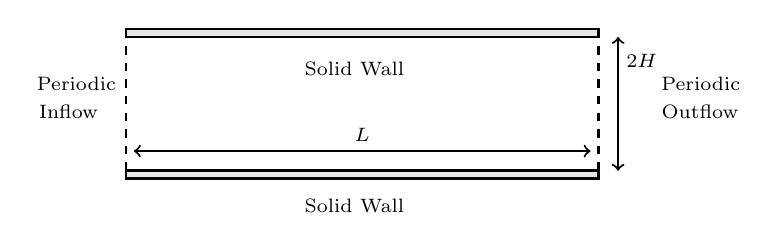
\begin{tikzpicture}
    % Draw a rectangle with specified properties
    \draw[line width=1pt, fill=gray!20] (0.0,1.8) rectangle (6.0,1.9);
    \draw[line width=1pt, fill=gray!20] (0.0,0.0) rectangle (6.0,0.1);
    \draw[dashed, line width=1pt] (0,0.1) -- (0,1.9);
    \draw[dashed, line width=1pt] (6,0.1) -- (6,1.9);
    
    \node at (2.6+0.3, 1.4) {\scriptsize Solid Wall};
    \node at (2.6+0.3, -0.35) {\scriptsize Solid Wall};
    
    \node at (-0.63, 1.2) {\scriptsize Periodic};
    \node at (-0.73, 0.85) {\scriptsize Inflow};
    
    \node at (7.15+0.15, 1.2) {\scriptsize Periodic};
    \node at (7.15+0.14, 0.85) {\scriptsize Outflow};
    
    % draw arrows
    \draw[<->, line width=0.75pt] (0.1, 0.35) -- (5.9, 0.35);
    \node at (3.0, 0.55) {\scriptsize $L$};
    \draw[<->, line width=0.75pt] (6.25, 0.1) -- (6.25, 1.8);
    \node at (6.55, 1.5) {\scriptsize $2H$};
    \end{tikzpicture}
    \captionsetup{width=0.85\textwidth}
    \caption{Computational domain for turbulent channel flow.}
    \label{fig:fully_developed_turbulent_channel_flow}
\end{figure}
The simulation is run at a Reynolds number $\text{Re}_H = 22000$ based on the half-channel height $H$.
However, in turbulence modelling and especially for turbulent channel flow, the friction Reynolds number ($\text{Re}_\tau $) given by $\text{Re}_\tau := (U_\tau H) / \nu $ is often used as a measure of the flow.
The simulation is run at $\text{Re}_\tau = 550$.
\begin{table}
    \centering
    \begin{tabular}{m{2.1cm} m{1.75cm} m{1.75cm} m{1.75cm} m{1.75cm}}
        \hline
        & $\mathbf{u}$ & $p$ & $k$ & $\varepsilon$ \\
        \hline
        \textbf{Inflow} & Periodic & $p=p_{\text{in}}$ & Periodic & periodic \\
        \textbf{Outflow} & Periodic & $p=p_\text{out}$ & Periodic & periodic \\
        \textbf{Solid walls} & $0$ & $\nabla p \cdot \mathbf{n} = 0$ & $0$ & $\nabla \varepsilon \cdot \mathbf{n} = 0$ \\
        \hline
    \end{tabular}
    \captionsetup{width=0.85\textwidth}
    \caption{Boundary conditions for turbulent channel flow.}
    \label{fig:fully_developed_turbulent_channel_flow}
\end{table}
To verify the model's accuracy, numerical results are compared to a direct numerical simulation performed by \cite{lee_direct_2015}.
The same simulation is conducted for a series of meshes with various values of $d^+$ ranging from $16$ to $0.5$ (with smaller values indicating a finer mesh), with the results provided in \cref{fig:channel_flow_profiles} (for better clarity, the results corresponding to some values of $d^+$ are not shown).
\begin{figure}[htbp]
    \centering
    \includegraphics[width=0.825\textwidth]{channel flow-profiles.pdf}
    \captionsetup{width=0.85\textwidth}
    \caption{Comparison of velocity (top) and turbulent kinetic energy (bottom) profiles obtained on meshes with different resolutions with direct numerical simulation (left), together with close-up plots (right).}
    \label{fig:channel_flow_profiles}
\end{figure}
Considering the solution profiles from \cref{fig:channel_flow_profiles} and the fact that the fields are most sensitive in the viscous sublayer, we feel that a value of $d^+ = 2$ strikes a good balance between computational efficiency and numerical accuracy.
In particular, the number of elements in this mesh is $864$.
The velocity and pressure spaces have $3,480$ and $511$ degrees of freedom, respectively. On the other hand, both the $k$ and $\varepsilon$ function spaces have $438$ degrees of freedom.
Since the results for meshes with values $d^+ = 2$ and $d^+ = 0.5$ do not differ dramatically, the former value will also be used when constructing a mesh for the next flow case.

\subsection{Flow over a Backward-Facing Step}
Flow over a backward-facing step occurs when a fluid flows over a sudden expansion, creating a separated flow region and a complex recirculation zone downstream of the step.
The domain and boundary conditions are constructed such that they match the data from the experiment performed by \cite{driver_features_1985}, which can be seen in \cref{fig:backward_facing_step} and \cref{tab: boundary conditions for the backward facing step}, respectively.
This is a significantly more complex scenario than the channel flow, making it a perfect model validation case.
Because of the mesh size, a steady-state solver was used.
\begin{figure}[htbp]
    \centering
    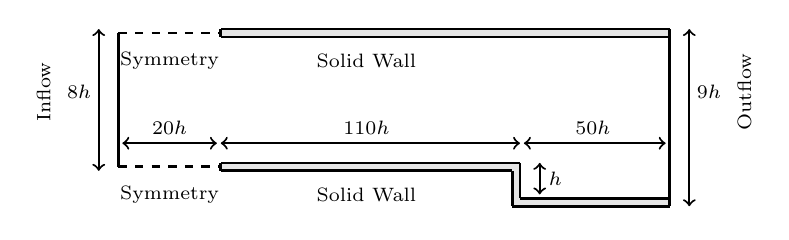
\begin{tikzpicture}
    
        \fill[gray!20] (2.3,1.7) rectangle (8.0,1.8);
        \draw[solid,  line width=1pt]     (2.3,1.7) -- (8.0,1.7);
        \draw[solid,  line width=1pt]     (8.0,1.7) -- (8.0,1.8);
        \draw[solid,  line width=1pt]     (8.0,1.8) -- (2.3,1.8);
        \draw[solid,  line width=1pt]     (2.3,1.8) -- (2.3,1.7);
        
        \fill[gray!20] (2.3,0.0) rectangle (6,0.1);
        \fill[gray!20] (6,-0.45) rectangle (8,-0.35);
        \fill[gray!20] (6,-0.45) rectangle (6.1,0.1);

        \draw[solid,  line width=1.0pt]     (2.3,0.0) -- (6.0,0.0);
        \draw[solid,  line width=1.0pt]     (6.0,0.0) -- (6.0, -0.45);
        \draw[solid,  line width=1.0pt]     (6.0, -0.45) -- (8.0, -0.45);
        \draw[solid,  line width=1.0pt]     (8.0, -0.45) -- (8.0, -0.35);
        \draw[solid,  line width=1.0pt]     (8.0, -0.35) -- (6.1, -0.35);
        \draw[solid,  line width=1.0pt]     (6.1, -0.35) -- (6.1, 0.1);
        \draw[solid,  line width=1.0pt]     (6.1, 0.1) -- (2.3, 0.1);
        \draw[solid,  line width=1.0pt]     (2.3, 0.1) -- (2.3, 0.0);

        \draw[dashed, line width=1pt]     (1.,1.75) -- (2.3,1.75);
        \draw[dashed, line width=1pt]     (1.,0.05) -- (2.3,0.05);
        \draw[solid,  line width=1pt]     (1.,0.05) -- (1.,1.75);
        \draw[solid,  line width=1pt]     (8,-0.35) -- (8,1.7);

        % Add text labels
        \node at (2.15+2.0, 1.4) {\scriptsize Solid Wall};
        \node at (2.15+2.0, -0.3) {\scriptsize Solid Wall};
        \node at (1.65, 1.4) {\scriptsize Symmetry};
        \node at (1.65, -0.3) {\scriptsize Symmetry};

        \node[rotate=90] at (0.05, 1.) {\scriptsize Inflow};
        \node[rotate=90] at (8.95, 1.) {\scriptsize Outflow};
        % draw arrows
        \draw[<->, line width=0.75pt] (6.35, 0.1) -- (6.35, -0.3);
        \node at (6.55, -0.1) {\scriptsize $h$};
 
        \draw[<->, line width=0.75pt] (1.05, 0.35) -- (2.25, 0.35);
        \node at (1.65, 0.55) {\scriptsize $20h$};
        
        \draw[<->, line width=0.75pt] (2.3, 0.35) -- (6.1, 0.35);
        \node at (4.15, 0.55) {\scriptsize $110h$};
        
        \draw[<->, line width=0.75pt] (6.15, 0.35) -- (7.95, 0.35);
        \node at (7.025, 0.55) {\scriptsize $50h$};

        \draw[<->, line width=0.75pt] (8.25, -0.45) -- (8.25, 1.8);
        \node at (8.5, 1.) {\scriptsize $9h$}; 
    
        \draw[<->, line width=0.75pt] (0.75, 0.0) -- (0.75, 1.8);
        \node at (0.5, 1.) {\scriptsize $8h$};
    \end{tikzpicture}
    \captionsetup{width=0.85\textwidth} 
    \caption{Computational domain for the flow over a backward-facing step.}
    \label{fig:backward_facing_step}
\end{figure}
The Reynolds number based on the step height $h$ is approximately $\text{Re}_h = 36,000$, where the reference velocity used to compute $\text{Re}_h$ is measured just before encountering the step, specifically at $x = -4h$ (with the step located at $x=0$).
The computational mesh consists of $129,844$ elements.
There are $523,038$ and $65,838$ degrees of freedom for the velocity and pressure spaces, respectively, and $65,838$ for both the $k$ and $\varepsilon$ spaces.
\begin{table}
    \centering
    \begin{tabular}{m{2.1cm} m{1.75cm} m{1.75cm} m{1.75cm} m{1.75cm}}
        \hline
        & $\mathbf{u}$ & $p$ & $k$ & $\varepsilon$ \\
        \hline
        \textbf{Inflow} & $\mathbf{u}_{\text{in}}$ & $\nabla p \cdot \mathbf{n} = 0$
        & $k_{\text{in}}$ & $\varepsilon_{\text{in}}$
        \\
        \textbf{Outflow} & $\nabla \mathbf{u} \cdot \mathbf{n} = 0$ & $p=0$
        & $\nabla k \cdot \mathbf{n} = 0$ & $\nabla \varepsilon\cdot \mathbf{n} = 0$
        \\
        \textbf{Solid walls} & $0$ & $\nabla p \cdot \mathbf{n} = 0$
        & $0$ & $\nabla \varepsilon \cdot \mathbf{n} = 0$
        \\
        \textbf{Symmetry} & $\mathbf{u} \cdot \mathbf{n} = 0$ & $\nabla p \cdot \mathbf{n} = 0$
        & $\nabla k \cdot \mathbf{n} = 0$ & $\nabla \varepsilon \cdot \mathbf{n} = 0$
        \\
        \hline
    \end{tabular}
    \captionsetup{width=0.85\textwidth}
    \caption{Boundary conditions for the flow over a backward-facing step.}
    \label{tab: boundary conditions for the backward facing step}
\end{table}

The model's accuracy is verified using experimental data from \cite{driver_features_1985}.
A key measure of success is the accurate prediction of the reattachment point downstream of the step.
This is determined by measuring the point $\hat{x}$ where the skin friction coefficient ($C_f$) is equal zero.
This was achieved in the experiment by using a laser oil flow interferometer. Another measure for analysing the results is the pressure coefficient ($C_p$).
The results in \cref{fig:backstep_coefficients} show a poor match between the simulation and the experiment, with the reattachment point observed at $\hat{x} = 6.26 h$, compared to the simulation's $\hat{x} = 5.0 h$.
However, this discrepancy is expected from the $k$-$\varepsilon$ model, which is known to struggle with separation and adverse pressure gradients.
When compared to results in \cite{steffen_jr._critical_1993} with multiple versions of the $k$-$\varepsilon$ model, with reattachment points ranging from $\hat{x} = 4.9$ to $\hat{x} = 5.5$, we see a better match.

\begin{figure}[htbp]
    \centering
    \includegraphics[width=0.825\textwidth]{backstep-coefficients.pdf}
    \captionsetup{width=0.85\textwidth}
    \caption{Comparison of the skin friction coefficient (left) and the pressure coefficient (right) between the experiment and simulation.}
    \label{fig:backstep_coefficients}
\end{figure}

\Cref{fig:backstep_profiles} presents normalized velocity magnitude $U/U_\infty$ and $k$ profiles at four points after the step.
Although the velocity profiles show good agreement, $k$ diverges after $x = 4h$, which is likely the cause of the reattachment point appearing prematurely.
\begin{figure}[htbp]
    \centering
    \includegraphics[width=0.825\textwidth]{backstep-profiles.pdf}
    \captionsetup{width=0.85\textwidth}
    \caption{Comparison of the velocity (top) and turbulent kinetic energy (bottom) profiles at $x = 1h$ (left), $x = 4h$ (second left), $x = 6h$ (second right), and $x = 10h$ (right) between the experiment and simulation.}
    \label{fig:backstep_profiles}
\end{figure}

% Section 4 - Conclusion
\section{Conclusion}
The LB $k$-$\varepsilon$ turbulence model was successfully implemented on the FEniCS computing platform, in both the transient and steady-state formulations.
We verified the implementation of the transient solver by simulating fully developed channel flow, where very good agreement was found between the computed solutions and the direct numerical simulation.
Although the results of the backward-facing step simulation did not match the experiment, we still consider the implementation of the steady-state solver a success, since the results matched the expected behaviour of the $k$-$\varepsilon$ model.
It is clear from those results that the working $k$-$\varepsilon$ model in FEniCS can be implemented with relative ease, and we see no reason why that would not be true for different turbulence models such as the $k$-$\omega$ or Spalart--Allmaras model.
These results can be replicated via scripts archived at \href{https://github.com/joove123/k-epsilon}{https://github.com/joove123/k-epsilon}.

\begin{acknowledgement}
    I would like to thank my master's thesis supervisor, Professor Achim Schroll, for professional guidance and support during the writing of my master's thesis and this article.
    I also thank NumFOCUS for the travel award that enabled me to attend the FEniCS 2024 conference.
\end{acknowledgement}
% ---- Article ends here ----
\bibliographystyle{spbasic}
% Write the full path of your bibfile relative to book.tex
\bibliography{chapters/marcibal/bibliography.bib}

